% Options for packages loaded elsewhere
\PassOptionsToPackage{unicode}{hyperref}
\PassOptionsToPackage{hyphens}{url}


\documentclass[
]{article}

%\usepackage{tcolorbox}
%\newtcolorbox{myquote}{colback=red!5!white, colframe=red!75!black}
%\newtcolorbox{myShaded}{colback=red!5!white, colframe=red!75!black}
% redefine the 'quote' environment to use this 'myquote' environment
%\renewenvironment{quote}{\begin{myquote}}{\end{myquote}}
%\newenvironment{Highlighting}{\begin{myquote}}{\end{myquote}}

\usepackage{lmodern}
\usepackage{amssymb,amsmath}


\usepackage{ifxetex,ifluatex}
\ifnum 0\ifxetex 1\fi\ifluatex 1\fi=0 % if pdftex
  \usepackage{mathpazo} % Palatino-like math fonts

  \usepackage[T1]{fontenc}
  \usepackage[utf8]{inputenc}
  \usepackage{textcomp} % provide euro and other symbols
\else % if luatex or xetex

% Load mathpazo as a math font
\usepackage{mathpazo}

% Load Pagella as a text font by specifying no-math to fontspec
%\usepackage[no-math]{fontspec}
%\setmainfont[Numbers=Proportional]{TeX Gyre Pagella}

  \usepackage{unicode-math}
  \defaultfontfeatures{Scale=MatchLowercase}
  \defaultfontfeatures[\rmfamily]{Ligatures=TeX,Scale=1}
  \setmainfont[Numbers = Proportional]{TeX Gyre Pagella}
  \setmonofont[]{Ubuntu Mono}
\fi
% Use upquote if available, for straight quotes in verbatim environments
\IfFileExists{upquote.sty}{\usepackage{upquote}}{}
\IfFileExists{microtype.sty}{% use microtype if available
  \usepackage[]{microtype}
  \UseMicrotypeSet[protrusion]{basicmath} % disable protrusion for tt fonts
}{}
\makeatletter
\@ifundefined{KOMAClassName}{% if non-KOMA class
  \IfFileExists{parskip.sty}{%
    \usepackage{parskip}
  }{% else
    \setlength{\parindent}{0pt}
    \setlength{\parskip}{6pt plus 2pt minus 1pt}}
}{% if KOMA class
  \KOMAoptions{parskip=half}}
\makeatother
\usepackage{xcolor}
\IfFileExists{xurl.sty}{\usepackage{xurl}}{} % add URL line breaks if available
\IfFileExists{bookmark.sty}{\usepackage{bookmark}}{\usepackage{hyperref}}
\hypersetup{
  pdftitle={Homework \#2},
  pdfauthor={Coffee Automaton},
  hidelinks,
  pdfcreator={LaTeX via pandoc}}
\urlstyle{same} % disable monospaced font for URLs
\usepackage[margin = 1in]{geometry}
\usepackage{color}
\usepackage{fancyvrb}
\newcommand{\VerbBar}{|}
\newcommand{\VERB}{\Verb[commandchars=\\\{\}]}
\DefineVerbatimEnvironment{Highlighting}{Verbatim}{commandchars=\\\{\}}
% Add ',fontsize=\small' for more characters per line
\usepackage{framed}
\definecolor{shadecolor}{RGB}{248,248,248}
\newenvironment{Shaded}{\begin{snugshade}}{\end{snugshade}}
\newcommand{\AlertTok}[1]{\textcolor[rgb]{0.94,0.16,0.16}{#1}}
\newcommand{\AnnotationTok}[1]{\textcolor[rgb]{0.56,0.35,0.01}{\textbf{\textit{#1}}}}
\newcommand{\AttributeTok}[1]{\textcolor[rgb]{0.77,0.63,0.00}{#1}}
\newcommand{\BaseNTok}[1]{\textcolor[rgb]{0.00,0.00,0.81}{#1}}
\newcommand{\BuiltInTok}[1]{#1}
\newcommand{\CharTok}[1]{\textcolor[rgb]{0.31,0.60,0.02}{#1}}
\newcommand{\CommentTok}[1]{\textcolor[rgb]{0.56,0.35,0.01}{\textit{#1}}}
\newcommand{\CommentVarTok}[1]{\textcolor[rgb]{0.56,0.35,0.01}{\textbf{\textit{#1}}}}
\newcommand{\ConstantTok}[1]{\textcolor[rgb]{0.00,0.00,0.00}{#1}}
\newcommand{\ControlFlowTok}[1]{\textcolor[rgb]{0.13,0.29,0.53}{\textbf{#1}}}
\newcommand{\DataTypeTok}[1]{\textcolor[rgb]{0.13,0.29,0.53}{#1}}
\newcommand{\DecValTok}[1]{\textcolor[rgb]{0.00,0.00,0.81}{#1}}
\newcommand{\DocumentationTok}[1]{\textcolor[rgb]{0.56,0.35,0.01}{\textbf{\textit{#1}}}}
\newcommand{\ErrorTok}[1]{\textcolor[rgb]{0.64,0.00,0.00}{\textbf{#1}}}
\newcommand{\ExtensionTok}[1]{#1}
\newcommand{\FloatTok}[1]{\textcolor[rgb]{0.00,0.00,0.81}{#1}}
\newcommand{\FunctionTok}[1]{\textcolor[rgb]{0.00,0.00,0.00}{#1}}
\newcommand{\ImportTok}[1]{#1}
\newcommand{\InformationTok}[1]{\textcolor[rgb]{0.56,0.35,0.01}{\textbf{\textit{#1}}}}
\newcommand{\KeywordTok}[1]{\textcolor[rgb]{0.13,0.29,0.53}{\textbf{#1}}}
\newcommand{\NormalTok}[1]{#1}
\newcommand{\OperatorTok}[1]{\textcolor[rgb]{0.81,0.36,0.00}{\textbf{#1}}}
\newcommand{\OtherTok}[1]{\textcolor[rgb]{0.56,0.35,0.01}{#1}}
\newcommand{\PreprocessorTok}[1]{\textcolor[rgb]{0.56,0.35,0.01}{\textit{#1}}}
\newcommand{\RegionMarkerTok}[1]{#1}
\newcommand{\SpecialCharTok}[1]{\textcolor[rgb]{0.00,0.00,0.00}{#1}}
\newcommand{\SpecialStringTok}[1]{\textcolor[rgb]{0.31,0.60,0.02}{#1}}
\newcommand{\StringTok}[1]{\textcolor[rgb]{0.31,0.60,0.02}{#1}}
\newcommand{\VariableTok}[1]{\textcolor[rgb]{0.00,0.00,0.00}{#1}}
\newcommand{\VerbatimStringTok}[1]{\textcolor[rgb]{0.31,0.60,0.02}{#1}}
\newcommand{\WarningTok}[1]{\textcolor[rgb]{0.56,0.35,0.01}{\textbf{\textit{#1}}}}
\usepackage{graphicx,grffile}
\makeatletter
\def\maxwidth{\ifdim\Gin@nat@width>\linewidth\linewidth\else\Gin@nat@width\fi}
\def\maxheight{\ifdim\Gin@nat@height>\textheight\textheight\else\Gin@nat@height\fi}
\makeatother
% Scale images if necessary, so that they will not overflow the page
% margins by default, and it is still possible to overwrite the defaults
% using explicit options in \includegraphics[width, height, ...]{}
\setkeys{Gin}{width=\maxwidth,height=\maxheight,keepaspectratio}
% Set default figure placement to htbp
\makeatletter
\def\fps@figure{htbp}
\makeatother
\setlength{\emergencystretch}{3em} % prevent overfull lines
\providecommand{\tightlist}{%
  \setlength{\itemsep}{0pt}\setlength{\parskip}{0pt}}
\setcounter{secnumdepth}{-\maxdimen} % remove section numbering

% text wrapping
\usepackage{fvextra}
\DefineVerbatimEnvironment{Highlighting}{Verbatim}{breaklines,commandchars=\\\{\}}
\renewenvironment{verbatim}{\begin{Shaded}}{\end{Shaded}}


\title{
  \vspace{2in}
  \textmd{\textbf{Homework \#2}}
  \normalsize\vspace{0.1in}\\
  \textmd{\textbf{CS 217 @ SJTU}}
  \normalsize\vspace{0.1in}\\
}

\author{Coffee Automaton}
\date{}

\begin{document}

\noindent
\large\textbf{Homework \#2}
\hfill
\textbf{Coffee Automaton} \\
\normalsize {\bf CS 217 @ SJTU} \hfill ACM Class, Zhiyuan College, SJTU\\
Prof.~{\bf Dominik Scheder} \hfill Due Date: October 7, 2019\\
  TA.~{\bf Tang Shuyang}
\hfill Submit Date: \today


\hypertarget{exercise-1}{%
\section{Exercise 1}\label{exercise-1}}

If we want to find the maximum item in \(n\) items, to ensure it is the
maximum, it should be compared with all others directly or indirectly,
so any algorithms should be at least \(n-1\) comparisons.

If not, there is no comparison between the ``maximum'' and some others,
and we can not ensure its correctness.

\hypertarget{exercise-2}{%
\section{Exercise 2}\label{exercise-2}}

Record the maximum and the minimum.

Fetch \(2\) items each time, compare them, compare the smaller item and
the minimum, and compare the bigger item and the maximum.

The algorithm shows below.

\begin{Shaded}
\begin{Highlighting}[]
\KeywordTok{def}\NormalTok{ exercise_2(a, n):  }\CommentTok{# a is the array, and n is the size}
    \ControlFlowTok{if}\NormalTok{ n }\OperatorTok{==} \DecValTok{1}\NormalTok{:}
        \ControlFlowTok{return}\NormalTok{ [a[}\DecValTok{0}\NormalTok{], a[}\DecValTok{0}\NormalTok{]]}
    \ControlFlowTok{elif}\NormalTok{ a[}\DecValTok{0}\NormalTok{] }\OperatorTok{<}\NormalTok{ a[}\DecValTok{1}\NormalTok{]:  }\CommentTok{# 1 comparison}
        \BuiltInTok{max} \OperatorTok{=}\NormalTok{ a[}\DecValTok{1}\NormalTok{]}
        \BuiltInTok{min} \OperatorTok{=}\NormalTok{ a[}\DecValTok{0}\NormalTok{]}
    \ControlFlowTok{else}\NormalTok{:}
        \BuiltInTok{max} \OperatorTok{=}\NormalTok{ a[}\DecValTok{0}\NormalTok{]}
        \BuiltInTok{min} \OperatorTok{=}\NormalTok{ a[}\DecValTok{1}\NormalTok{]}
    \ControlFlowTok{for}\NormalTok{ i }\KeywordTok{in} \BuiltInTok{range}\NormalTok{(}\DecValTok{1}\NormalTok{, n }\OperatorTok{//} \DecValTok{2}\NormalTok{):  }\CommentTok{# 3 comparisons for each cycle}
        \ControlFlowTok{if}\NormalTok{ a[}\DecValTok{2} \OperatorTok{*}\NormalTok{ i] }\OperatorTok{<}\NormalTok{ a[}\DecValTok{2} \OperatorTok{*}\NormalTok{ i }\OperatorTok{+} \DecValTok{1}\NormalTok{]:}
\NormalTok{            l }\OperatorTok{=}\NormalTok{ a[}\DecValTok{2} \OperatorTok{*}\NormalTok{ i]}
\NormalTok{            r }\OperatorTok{=}\NormalTok{ a[}\DecValTok{2} \OperatorTok{*}\NormalTok{ i }\OperatorTok{+} \DecValTok{1}\NormalTok{]}
        \ControlFlowTok{else}\NormalTok{:}
\NormalTok{            l }\OperatorTok{=}\NormalTok{ a[}\DecValTok{2} \OperatorTok{*}\NormalTok{ i }\OperatorTok{+} \DecValTok{1}\NormalTok{]}
\NormalTok{            r }\OperatorTok{=}\NormalTok{ a[}\DecValTok{2} \OperatorTok{*}\NormalTok{ i]}
        \ControlFlowTok{if}\NormalTok{ l }\OperatorTok{<} \BuiltInTok{min}\NormalTok{:}
            \BuiltInTok{min} \OperatorTok{=}\NormalTok{ l}
        \ControlFlowTok{if}\NormalTok{ r }\OperatorTok{>} \BuiltInTok{max}\NormalTok{:}
            \BuiltInTok{max} \OperatorTok{=}\NormalTok{ r}
  
    \ControlFlowTok{return}\NormalTok{ [}\BuiltInTok{max}\NormalTok{, }\BuiltInTok{min}\NormalTok{]}
  
\end{Highlighting}
\end{Shaded}

The algorithm all use \(1+(\frac{n-2}{2})\times 3=\frac{3n}{2}-2\)
comparisons.

\hypertarget{exercise-3}{%
\section{Exercise 3}\label{exercise-3}}

Each time compare two items, take the larger one to the next round, and
after \(k-1\) rounds, there are two items. Compare them, and get the
``max'' and the ``second''.

Then find the items those were compared with the ``max'', compare them
with ``second''. the maximum is the second largest item.

The algorithm shows below.

\begin{Shaded}
\begin{Highlighting}[]
\ImportTok{import}\NormalTok{ numpy }\ImportTok{as}\NormalTok{ np}
  
\KeywordTok{def}\NormalTok{ exercise_3(a, n, k):  }\CommentTok{# a is the array, and n is the size n = 2^k}
\NormalTok{    l }\OperatorTok{=}\NormalTok{ np.zeros(n, k)}
\NormalTok{    b }\OperatorTok{=}\NormalTok{ np.zeros(n)}
    \ControlFlowTok{for}\NormalTok{ i }\KeywordTok{in} \BuiltInTok{range}\NormalTok{(}\DecValTok{0}\NormalTok{, n):}
\NormalTok{        b[i] }\OperatorTok{=}\NormalTok{ i}
\NormalTok{    m }\OperatorTok{=}\NormalTok{ n }\OperatorTok{//} \DecValTok{2}
    \ControlFlowTok{for}\NormalTok{ i }\KeywordTok{in} \BuiltInTok{range}\NormalTok{(}\DecValTok{0}\NormalTok{, k }\OperatorTok{-} \DecValTok{1}\NormalTok{):  }\CommentTok{# 2^(k-i-1) comparisons}
        \ControlFlowTok{for}\NormalTok{ j }\KeywordTok{in} \BuiltInTok{range}\NormalTok{(}\DecValTok{0}\NormalTok{, m):}
            \ControlFlowTok{if}\NormalTok{ a[b[j]] }\OperatorTok{<}\NormalTok{ a[b[j }\OperatorTok{+} \DecValTok{1}\NormalTok{]]:}
\NormalTok{                l[b[j }\OperatorTok{+} \DecValTok{1}\NormalTok{]].append(b[j])}
\NormalTok{                b.pop(j)}
            \ControlFlowTok{else}\NormalTok{:}
\NormalTok{                l[b[j]].append(b[j }\OperatorTok{+} \DecValTok{1}\NormalTok{])}
\NormalTok{                b.pop(j }\OperatorTok{+} \DecValTok{1}\NormalTok{)}
\NormalTok{    m }\OperatorTok{=}\NormalTok{ m }\OperatorTok{//} \DecValTok{2}
    \ControlFlowTok{if}\NormalTok{ a[b[}\DecValTok{0}\NormalTok{]] }\OperatorTok{<}\NormalTok{ a[b[}\DecValTok{1}\NormalTok{]]:  }\CommentTok{# 1 comparison}
        \BuiltInTok{max} \OperatorTok{=}\NormalTok{ a[b[}\DecValTok{1}\NormalTok{]]}
\NormalTok{        second }\OperatorTok{=}\NormalTok{ a[b[}\DecValTok{0}\NormalTok{]]}
\NormalTok{        compare }\OperatorTok{=}\NormalTok{ l[b[}\DecValTok{1}\NormalTok{]]}
    \ControlFlowTok{else}\NormalTok{:}
        \BuiltInTok{max} \OperatorTok{=}\NormalTok{ a[b[}\DecValTok{0}\NormalTok{]]}
\NormalTok{        second }\OperatorTok{=}\NormalTok{ a[b[}\DecValTok{1}\NormalTok{]]}
\NormalTok{        compare }\OperatorTok{=}\NormalTok{ l[b[}\DecValTok{0}\NormalTok{]]}
    \ControlFlowTok{for}\NormalTok{ i }\KeywordTok{in} \BuiltInTok{range}\NormalTok{(}\DecValTok{0}\NormalTok{, k):  }\CommentTok{# k comparisons}
        \ControlFlowTok{if}\NormalTok{ a[compare[i]] }\OperatorTok{>}\NormalTok{ second:}
\NormalTok{            second }\OperatorTok{=}\NormalTok{ a[compare[i]]}
  
\end{Highlighting}
\end{Shaded}

It all uses
\(\frac{n}{2}+\frac{n}{4}+\cdots+2+1+(k-1)=n+k-2=n+\log_2(n)-2\)
comparisons.

\hypertarget{exercise-4}{%
\section{Exercise 4}\label{exercise-4}}

Set the expected number of comparisons as \(S\).

\[\begin{aligned}
S&=\mathbf{E}[\sum_{i\neq j} A_{i,j}]\\
&=\sum_{i\neq j}\mathbf{E}[A_{i,j}]\\
&=\sum_{i}\sum_{j}\frac{1}{|i-j|+1}-n
\end{aligned}\]

Now considering the summation,as matrix (1) shows, the summation of the
matrix equals the summation.

\[\begin{aligned}
\begin{pmatrix}
1&\cfrac{1}{2}&\cfrac{1}{3}&\cdots& &\cfrac{1}{n}\\
\cfrac{1}{2}&1&\cfrac{1}{2}&\cdots&&\cfrac{1}{n-1}\\\cdots
& &...\\
\cfrac{1}{n-1}&\cfrac{1}{n-2}& &\cdots&1&\cfrac{1}{2}\\
\cfrac{1}{n}&1&\cfrac{1}{n-1}&\cdots&\cfrac{1}{2}&1\\
\end{pmatrix}
\end{aligned}\]

Using the Harmonic number \(H_{n}=1+\frac{1}{2}+\cdots+\frac{1}{n}\)

\[\begin{aligned}
S&=\sum_{i}\sum_{j}\frac{1}{|i-j|+1}-n\\
&=n\times 1+2\times(n-1)\times\frac{1}{2}+2\times(n-2)\times\frac{1}{3}+\cdots+2\times(n-(n-1))\times\frac{1}{n}-n\\
&=2\left(\frac{n}{2}+\frac{n}{3}+\cdots+\frac{n}{n}-\frac{1}{2}-\frac{2}{3}-\cdots-\frac{n-1}{n}\right)\\
&=2\left(n\left(\frac{1}{2}+\frac{1}{3}+\cdots+\frac{1}{n})-(\frac{1}{2}+\frac{2}{3}+\cdots+\frac{n-1}{n}\right)\right)\\
&=2\left(n\left(H_{n}-1\right)-\left(\left(1-1\right)+\left(1-\frac{1}{2}\right)+\left(1-\frac{1}{3}\right)+\cdots+\left(1-\frac{1}{n}\right)\right)\right)\\
&=2\left(n\left(H_{n}-1\right)-\left(n-H_{n}\right)\right)\\
&=2\left(n+1\right)H_{n}-4n
\end{aligned}\]

Which is the expected number of comparisons.

\hypertarget{exercise-5}{%
\section{Exercise 5}\label{exercise-5}}

The QuickSelect method first chooses a random pivot \(k\), and divide
the array into \(k\) and two parts: bigger than \(k\), smaller than
\(k\), which is same as quicksort.

However, quickselect only concern one of the two parts, and omit the
other, while quicksort concern the both. So we can say that quickselect
is a ``partial execution'' of quicksort.

The example quicksort tree to find \(4\) shows in Figure 1, and the red
part is visited by quickselect.

\begin{figure}
\centering
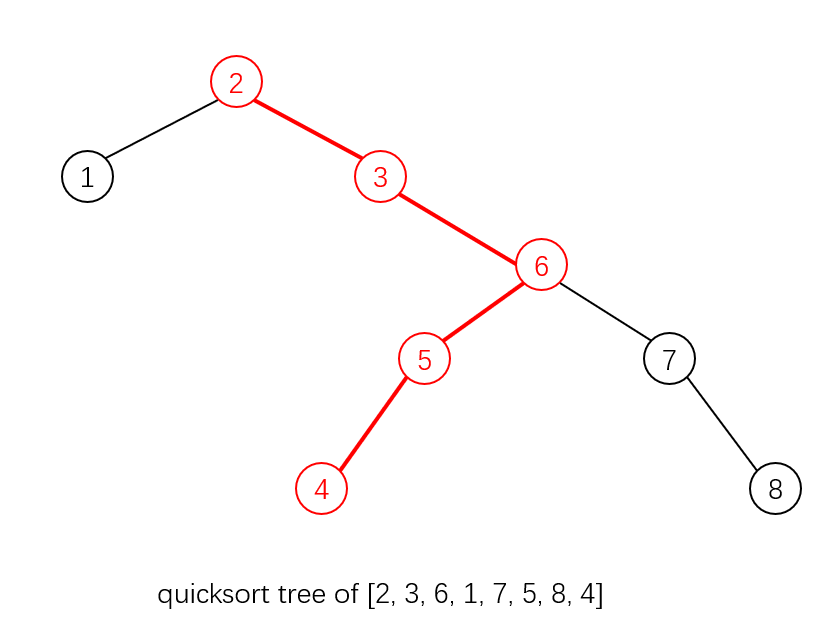
\includegraphics[width=0.5\textwidth,height=\textheight]{1.png}
\caption{The quicksort tree in Exercise 5}
\end{figure}

\hypertarget{exercise-6}{%
\section{Exercise 6}\label{exercise-6}}

If \(\mathbf{E}[B_{i,j,k}]=1\), then \(k\) is the ancestor of \(i\) and
\(j\).

Considering the Lemma of \(A_{i,j}\):\(A_{i,j}=1\) if and only if among
the elements of \([i:j]\), element i comes first in the input array.

So, \(B_{i,j,k}=1\) if and only if i comes first in \([i,j]\) and
\([i,k]\).

The length of section is \(\max(i,j,k)-\min(i,j,k)\), so
\(B_{i,j,k}=\dfrac{1}{\max(i,j,k)-\min(i,j,k)+1}\).

\[\mathbf E(B_{i,j,k})=\frac{1}{\max(i,j,k)-\min(i,j,k)+1}\]

\hypertarget{exercise-7}{%
\section{Exercise 7}\label{exercise-7}}

\[C(\pi,k)=\sum_{i\neq j} B_{i,j,k}\]

\hypertarget{exercise-8}{%
\section{Exercise 8}\label{exercise-8}}

\[\begin{aligned}
\mathbf E(C(\pi,1))&=\mathbf E\left(\sum_{i\neq j} B_{i,j,1}\right)\\
&=\sum_{i\neq j}\dfrac{1}{\max(i,j)}\\
&=2n-H(n)\\
&=2n-\ln n+o(1)
\end{aligned}\]

\hypertarget{exercise-9}{%
\section{Exercise 9}\label{exercise-9}}

\[\begin{aligned}
\mathbf{E}_{\pi}[C(\pi,k)]
&=\sum_{i\neq j}\frac{1}{\max(i,j,k)-\min(i,j,k)+1}\\
&=2n-H(k)-H(n-k+1)+2\sum_{i=1}^{n-k}\left(H(k+i)-H(i+1)\right)\\
&=2\left(n+\ln\frac{n!}{k!(n-k)!}-\ln k-\ln(n-k+1)\right)+o(n)
\end{aligned}\]

By the Stirling's formula, we have

\[\begin{aligned}
\mathbf{E}_{\pi}[C(\pi,k)]
&=2\left(n+n\ln n-k\ln k-(n-k)\ln(n-k)\right)+o(n)\\
&=2n(1-\kappa\ln\kappa-(1-\kappa)\ln(1-\kappa))+o(n)
\end{aligned}\]

\end{document}
